\documentclass[american,]{article}
\usepackage{lmodern}
\usepackage{amssymb,amsmath}
\usepackage{ifxetex,ifluatex}
\usepackage{fixltx2e} % provides \textsubscript
\ifnum 0\ifxetex 1\fi\ifluatex 1\fi=0 % if pdftex
  \usepackage[T1]{fontenc}
  \usepackage[utf8]{inputenc}
\else % if luatex or xelatex
  \ifxetex
    \usepackage{mathspec}
  \else
    \usepackage{fontspec}
  \fi
  \defaultfontfeatures{Ligatures=TeX,Scale=MatchLowercase}
\fi
% use upquote if available, for straight quotes in verbatim environments
\IfFileExists{upquote.sty}{\usepackage{upquote}}{}
% use microtype if available
\IfFileExists{microtype.sty}{%
\usepackage{microtype}
\UseMicrotypeSet[protrusion]{basicmath} % disable protrusion for tt fonts
}{}
\usepackage[margin=1in]{geometry}
\usepackage{hyperref}
\hypersetup{unicode=true,
            pdftitle={Regression Analysis of the Ames, Iowa Dataset},
            pdfauthor={Stuart Miller, Paul Adams, and Chance Robinson},
            pdfborder={0 0 0},
            breaklinks=true}
\urlstyle{same}  % don't use monospace font for urls
\ifnum 0\ifxetex 1\fi\ifluatex 1\fi=0 % if pdftex
  \usepackage[shorthands=off,main=american]{babel}
\else
  \usepackage{polyglossia}
  \setmainlanguage[variant=american]{english}
\fi
\usepackage{natbib}
\bibliographystyle{apalike}
\usepackage{color}
\usepackage{fancyvrb}
\newcommand{\VerbBar}{|}
\newcommand{\VERB}{\Verb[commandchars=\\\{\}]}
\DefineVerbatimEnvironment{Highlighting}{Verbatim}{commandchars=\\\{\}}
% Add ',fontsize=\small' for more characters per line
\usepackage{framed}
\definecolor{shadecolor}{RGB}{248,248,248}
\newenvironment{Shaded}{\begin{snugshade}}{\end{snugshade}}
\newcommand{\AlertTok}[1]{\textcolor[rgb]{0.94,0.16,0.16}{#1}}
\newcommand{\AnnotationTok}[1]{\textcolor[rgb]{0.56,0.35,0.01}{\textbf{\textit{#1}}}}
\newcommand{\AttributeTok}[1]{\textcolor[rgb]{0.77,0.63,0.00}{#1}}
\newcommand{\BaseNTok}[1]{\textcolor[rgb]{0.00,0.00,0.81}{#1}}
\newcommand{\BuiltInTok}[1]{#1}
\newcommand{\CharTok}[1]{\textcolor[rgb]{0.31,0.60,0.02}{#1}}
\newcommand{\CommentTok}[1]{\textcolor[rgb]{0.56,0.35,0.01}{\textit{#1}}}
\newcommand{\CommentVarTok}[1]{\textcolor[rgb]{0.56,0.35,0.01}{\textbf{\textit{#1}}}}
\newcommand{\ConstantTok}[1]{\textcolor[rgb]{0.00,0.00,0.00}{#1}}
\newcommand{\ControlFlowTok}[1]{\textcolor[rgb]{0.13,0.29,0.53}{\textbf{#1}}}
\newcommand{\DataTypeTok}[1]{\textcolor[rgb]{0.13,0.29,0.53}{#1}}
\newcommand{\DecValTok}[1]{\textcolor[rgb]{0.00,0.00,0.81}{#1}}
\newcommand{\DocumentationTok}[1]{\textcolor[rgb]{0.56,0.35,0.01}{\textbf{\textit{#1}}}}
\newcommand{\ErrorTok}[1]{\textcolor[rgb]{0.64,0.00,0.00}{\textbf{#1}}}
\newcommand{\ExtensionTok}[1]{#1}
\newcommand{\FloatTok}[1]{\textcolor[rgb]{0.00,0.00,0.81}{#1}}
\newcommand{\FunctionTok}[1]{\textcolor[rgb]{0.00,0.00,0.00}{#1}}
\newcommand{\ImportTok}[1]{#1}
\newcommand{\InformationTok}[1]{\textcolor[rgb]{0.56,0.35,0.01}{\textbf{\textit{#1}}}}
\newcommand{\KeywordTok}[1]{\textcolor[rgb]{0.13,0.29,0.53}{\textbf{#1}}}
\newcommand{\NormalTok}[1]{#1}
\newcommand{\OperatorTok}[1]{\textcolor[rgb]{0.81,0.36,0.00}{\textbf{#1}}}
\newcommand{\OtherTok}[1]{\textcolor[rgb]{0.56,0.35,0.01}{#1}}
\newcommand{\PreprocessorTok}[1]{\textcolor[rgb]{0.56,0.35,0.01}{\textit{#1}}}
\newcommand{\RegionMarkerTok}[1]{#1}
\newcommand{\SpecialCharTok}[1]{\textcolor[rgb]{0.00,0.00,0.00}{#1}}
\newcommand{\SpecialStringTok}[1]{\textcolor[rgb]{0.31,0.60,0.02}{#1}}
\newcommand{\StringTok}[1]{\textcolor[rgb]{0.31,0.60,0.02}{#1}}
\newcommand{\VariableTok}[1]{\textcolor[rgb]{0.00,0.00,0.00}{#1}}
\newcommand{\VerbatimStringTok}[1]{\textcolor[rgb]{0.31,0.60,0.02}{#1}}
\newcommand{\WarningTok}[1]{\textcolor[rgb]{0.56,0.35,0.01}{\textbf{\textit{#1}}}}
\usepackage{longtable,booktabs}
\usepackage{graphicx,grffile}
\makeatletter
\def\maxwidth{\ifdim\Gin@nat@width>\linewidth\linewidth\else\Gin@nat@width\fi}
\def\maxheight{\ifdim\Gin@nat@height>\textheight\textheight\else\Gin@nat@height\fi}
\makeatother
% Scale images if necessary, so that they will not overflow the page
% margins by default, and it is still possible to overwrite the defaults
% using explicit options in \includegraphics[width, height, ...]{}
\setkeys{Gin}{width=\maxwidth,height=\maxheight,keepaspectratio}
\IfFileExists{parskip.sty}{%
\usepackage{parskip}
}{% else
\setlength{\parindent}{0pt}
\setlength{\parskip}{6pt plus 2pt minus 1pt}
}
\setlength{\emergencystretch}{3em}  % prevent overfull lines
\providecommand{\tightlist}{%
  \setlength{\itemsep}{0pt}\setlength{\parskip}{0pt}}
\setcounter{secnumdepth}{5}
% Redefines (sub)paragraphs to behave more like sections
\ifx\paragraph\undefined\else
\let\oldparagraph\paragraph
\renewcommand{\paragraph}[1]{\oldparagraph{#1}\mbox{}}
\fi
\ifx\subparagraph\undefined\else
\let\oldsubparagraph\subparagraph
\renewcommand{\subparagraph}[1]{\oldsubparagraph{#1}\mbox{}}
\fi

%%% Use protect on footnotes to avoid problems with footnotes in titles
\let\rmarkdownfootnote\footnote%
\def\footnote{\protect\rmarkdownfootnote}

%%% Change title format to be more compact
\usepackage{titling}

% Create subtitle command for use in maketitle
\newcommand{\subtitle}[1]{
  \posttitle{
    \begin{center}\large#1\end{center}
    }
}

\setlength{\droptitle}{-2em}

  \title{Regression Analysis of the Ames, Iowa Dataset}
    \pretitle{\vspace{\droptitle}\centering\huge}
  \posttitle{\par}
    \author{Stuart Miller, Paul Adams, and Chance Robinson}
    \preauthor{\centering\large\emph}
  \postauthor{\par}
      \predate{\centering\large\emph}
  \postdate{\par}
    \date{Master of Science in Data Science, Southern Methodist University, USA}

\usepackage{booktabs}
\usepackage{longtable}
\usepackage{array}
\usepackage{multirow}
\usepackage[table]{xcolor}
\usepackage{wrapfig}
\usepackage{float}
\usepackage{colortbl}
\usepackage{pdflscape}
\usepackage{tabu}
\usepackage{threeparttable}
\usepackage{threeparttablex}
\usepackage[normalem]{ulem}
\usepackage{makecell}

\usepackage{amsmath}
\usepackage[utf8]{inputenc}
\usepackage[T1]{fontenc}
\usepackage{setspace}
\usepackage{hyperref}
\onehalfspacing
\setcitestyle{numbers,square,super}
\newcommand\numberthis{\addtocounter{equation}{1}\tag{\theequation}}

\begin{document}
\maketitle

\hypertarget{introduction}{%
\section{Introduction}\label{introduction}}

What is the price of a home in Ames, Iowa? Our inaugural project in the
program curriculum had us competing in an online competition utilizing
the linear regression techniques that we've learned up to this point.
Our team chose R as the preferred analysis platform as the consensus was
that it had more applicable uses in industry. The objective was to apply
various predictive models in order to assess the suitability of our
parameter selections in determining the sales price of a home. The
measure of accuracy was logged in terms of the Root Mean Square Error,
or RMSE, as well as other comparison models such as cross-validation and
the adjusted R-squared. Our approach was limited in that we not
permitted to use more advanced algorithms that we will be exposed to
later on, but the exploratory data analysis and data cleaning methods
that we've learned and made use of here will surely be of use to us in
our future personal and academic endeavors.

\hypertarget{ames-iowa-data-set}{%
\section{Ames, Iowa Data Set}\label{ames-iowa-data-set}}

The Ames, Iowa Data Set describes the sale of individual residential
properities from 2006-2010 in Ames, Iowa \cite{Cock}. The data was
retreved from the dataset hosting site Kaggle, where it is listed under
a machine learning competition named
\href{https://www.kaggle.com/c/house-prices-advanced-regression-techniques/overview}{\textit{House Prices: Advanced Regression Techniques}}
\cite{Kaggle2016}. The data is comprised of 37 numeric features, 43
non-numeric features and an observation index split between a training
set and a testing set, which contain 1460 and 1459 observations,
respectively. The response variable (\texttt{SalePrice}) is only
provided for the training set. The output of a model on the test set can
be submitted to the Kaggle competition for scoring the performance of
the model in terms of RMSE. The first analysis models property sale
prices (\texttt{SalePrice}) as the response of living room area
(\texttt{GrLivArea}) of the property and neighborhood
(\texttt{Neighborhood}) where it is located. In the second analysis,
variable selection techniques are used to determine which explanatory
varaibles are associated with \texttt{SalePrice} to find a predictive
model.

\hypertarget{analysis-question-i}{%
\section{Analysis Question I}\label{analysis-question-i}}

\hypertarget{question-of-interest}{%
\subsection{Question of Interest}\label{question-of-interest}}

Century 21 has commissioned an analysis of this data to determine how
the sale price of property is related to living room area of the
property in the Edwards, Northwest Ames, and Brookside neighborhoods of
Ames, IA.

\hypertarget{modeling}{%
\subsection{Modeling}\label{modeling}}

Linear regression will be used to model sale price as a response of the
living room area. From the initial exploratory data analysis, it was
determined that sale prices should be log-transformed to meet the model
assumptions for linearity (see section \ref{appendix:linearity}), thus
improving our models fit and reducing standard error. Additionally, two
observations were removed as they appeared to be from a different
population than the other observations in the dataset (see section
\ref{appendix:infleu-points}); therefore, analysis only considers
properties with living rooms less than 3500 sq. ft. in area.

We will consider two models: the logarithm of sale price as the response
of living room area (1), the reduced model, and the logarithm of sale
price as the response of living room area accounting for differences in
the three neighborhood of interest (Brookside, Northwest Ames, and
Edwards) where Edwards will be used as the reference (2), the full
model. An extra sums of square (ESS) test will be used to verify that
the addition of \texttt{Neighborhood} improves the model.

\textbf{Reduced Model}

\begin{equation}
\mu \lbrace log(SalePrice) \rbrace = \beta_0 + \beta_1(LivingRoomArea) \label{eq:reduced}
\end{equation}

\textbf{Full Model}

\begin{align}
\mu \lbrace log(SalePrice) \rbrace = \beta_0 + \beta_1(LivingRoomArea) +  \beta_2(Brookside) +\beta_3(NorthwestAmes) + \nonumber\\
\beta_3(Brookside)(LivingRoomArea) + \beta_4(NorthwestAmes)(LivingRoomArea) \label{eq:full}
\end{align}

The ESS test provides convincing evidence that the interaction terms are
useful for the model (p-value \textless{} 0.0001); thus, we will
continue with the full model.

\begin{verbatim}
## Analysis of Variance Table
## 
## Model 1: log(SalePrice) ~ (GrLivArea) + Neighborhood_BrkSide + Neighborhood_NAmes
## Model 2: log(SalePrice) ~ (GrLivArea) + Neighborhood_BrkSide + Neighborhood_NAmes + 
##     (GrLivArea) * Neighborhood_BrkSide + (GrLivArea) * Neighborhood_NAmes
##   Res.Df    RSS Df Sum of Sq      F    Pr(>F)    
## 1    377 14.824                                  
## 2    375 13.441  2    1.3834 19.299 1.053e-08 ***
## ---
## Signif. codes:  0 '***' 0.001 '**' 0.01 '*' 0.05 '.' 0.1 ' ' 1
\end{verbatim}

\hypertarget{model-assumptions-assessment}{%
\subsection{Model Assumptions
Assessment}\label{model-assumptions-assessment}}

The following assessments for model assumptions are made based on Figure
\ref{fig:diag-plots} and Figure \ref{fig:scatter-plots}:

\begin{itemize}
\tightlist
\item
  The residuals of the model appear to be approximately normally
  distrubited based on the QQ plot of the residuals and histogram of the
  residuals, suggesting the assumption of normality is met.
\item
  No patterns are evident in the scatter plots of residuals and
  studentized residuals vs predicted value, suggesting the assumption of
  constant variance is met.
\item
  While some observations appear to be influential and have high
  leverage, removing these observations does not have a significant
  impact on the result of the model fit.
\item
  Based on the scatter plot of the log transform of \texttt{SalePrice}
  vs \texttt{GrLivArea}, it appears that a linear model is reasonable
  (see section \ref{appendix:linearity}).
\end{itemize}

The sampling procedure is not known. We will assume the independence
assumption is met.

\begin{figure}[htbp]

{\centering 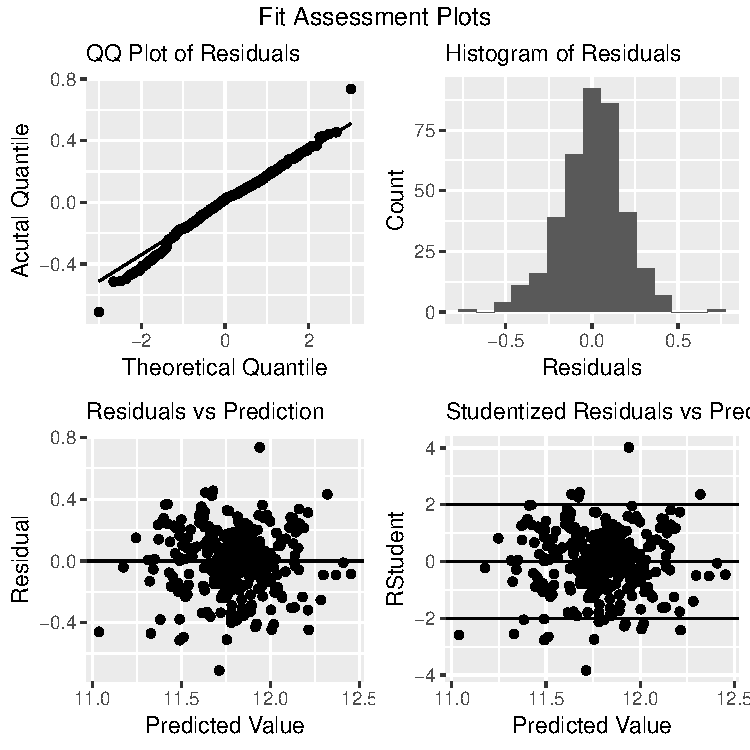
\includegraphics[width=0.45\linewidth]{HousePriceRegressionAnalysis_files/figure-latex/diag-plots-1} 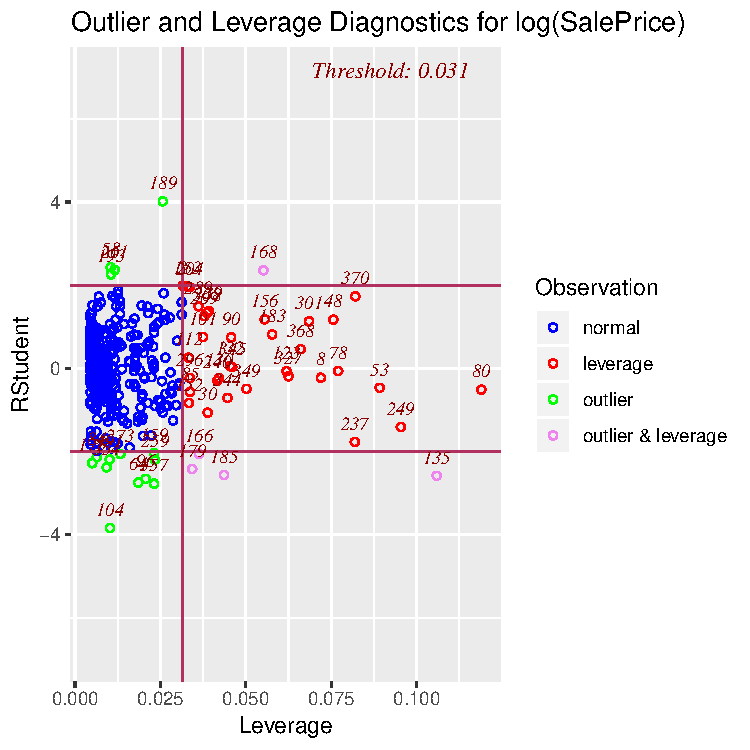
\includegraphics[width=0.45\linewidth]{HousePriceRegressionAnalysis_files/figure-latex/diag-plots-2} 

}

\caption{Diagnostic Plots}\label{fig:diag-plots}
\end{figure}

\hypertarget{comparing-competing-models}{%
\subsection{Comparing Competing
Models}\label{comparing-competing-models}}

The two models were trained and validated on the training dataset using
10-fold cross validation. The table below summerizes the performance of
the models with RMSE, adjusted \(R^2\), and PRESS. These results show
that the full model is an improvement over the reduced model, which is
consistent with the result of the ESS test.

\begin{table}[H]
\centering
\begin{tabular}{lrrr}
\toprule
Model & RMSE & CV.Press & Adjused.R.Squared\\
\midrule
Full Model & 0.1910566 & 12.51675 & 0.5084024\\
Reduced Model & 0.1988473 & 13.55835 & 0.4750767\\
\bottomrule
\end{tabular}
\end{table}

\hypertarget{parameters}{%
\subsection{Parameters}\label{parameters}}

The following table summerizes the parameter estimates for the full
model.

\begin{table}[H]
\centering
\begin{tabular}{lrrr}
\toprule
Parameter & Estimate & CI.Lower & CI.Upper\\
\midrule
Intercept & 11.0254845 & 10.8861855 & 11.1647836\\
GrLivArea & 0.0005387 & 0.0004324 & 11.1647836\\
Neighborhood\_BrkSide & -0.2338906 & -0.4468114 & -0.0209698\\
Neighborhood\_NAmes & 0.4178562 & 0.2558923 & 0.5798200\\
GrLivArea:Neighborhood\_BrkSide & 0.0001996 & 0.0000336 & 0.0003656\\
GrLivArea:Neighborhood\_NAmes & -0.0002145 & -0.0003366 & -0.0000924\\
\bottomrule
\end{tabular}
\end{table}

Where \texttt{Intercept} is \(\beta_0\), \texttt{GrLivArea} is
\(\beta_1\), \texttt{Neighborhood\_BrkSide} is \(\beta_2\),
\texttt{Neighborhood\_NAmes} is \(\beta_3\),
\texttt{GrLivArea:Neighborhood\_BrkSide} is \(\beta_4\), and
\texttt{GrLivArea:Neighborhood\_NAmes} is \(\beta_5\)

\hypertarget{model-interpretation}{%
\subsection{Model Interpretation}\label{model-interpretation}}

We estimate that for increase in 100 sq. ft., there is associated
multiplicative increase in median price of

\begin{itemize}
\tightlist
\item
  1.055 for the Edwards neighborhood with a 95\% confidence interval of
  {[}1.044 , 1.066{]}
\item
  1.033 for the Northwest Ames neighorhood with a 95\% confidence
  interval of {[}1.026 , 1.040{]}
\item
  1.077 for the Brookside neighorhood with a 95\% confidence interval of
  {[}1.063 , 1.090{]}
\end{itemize}

Since the sampling procedure is not known and this is an observational
study, the results only apply to this data.

\hypertarget{conclusion}{%
\subsection{Conclusion}\label{conclusion}}

In response to the analysis commissioned by Century 21, the log
transform of property sale price was modeled as a linear response to the
property living room area for residential properties in Ames, IA. It was
determined that it was necessary to include interaction terms to allow
for the influence of neighborhood on sale price. Based on the model,
there is strong evidence of an associated multiplicative increase in
median sale price for an increase in living room area (p-vlue
\textless{} 0.0001, overall F-test).

\hypertarget{analysis-question-ii}{%
\section{Analysis Question II}\label{analysis-question-ii}}

\hypertarget{question-of-interest-1}{%
\subsection{Question of Interest}\label{question-of-interest-1}}

Century 21 has commissioned a second analysis using the same data set,
expanded to include as many of the 80 total features, plus the index
split, as required to determine the sale price of residential properties
across all neighborhoods of Ames, Iowa, beyond only the three - Edwards,
Northwest Ames, and Brookside - previously commissioned for analysis.

\hypertarget{modeling-1}{%
\subsection{Modeling}\label{modeling-1}}

Through analyzing our variable selection and cross-validation processes
- along with our nascant domain knowledge of residential real estate -
we ultimately arrived at a multiple linear regression model featuring 11
linear predictor variables and two interaction terms. Specifically, our
variable selection process included direct analysis of a correlation
plot and a correlation matrix as well as performing forward selection,
backward elimination, and stepwise regression.

Regarding missing data, we imputed NA values for 19 variables using a
combination of the data dictionary provided by Century 21 as well as our
domain knowledge. After building models with and without transformations
applied to variables, we noted no significaznt difference in variable
selection from our selection process so elected to use non-transformed
predictor variables. We did, however, use the log-transformed
\texttt{SalePrice} applied in the first analysis.

\textbf{Forward Selection}

Forward selection is a variable selection methodology that begins with a
constant mean and adds explanatory variables one-by-one until no further
additonal predictor variables significantly improve the model's fit.
This employess the ``F-to-enter'' method from the extra-sum-of-squares
F-statistic. This was the first method we employed. For this process, we
provided the test a starting model with no predictor variables and a
model from which terms can be selected, which included all predictor
variables available. The process worked forward with selecting one
parameter. The suggested model shown in section
\ref{appendix:forSelection}.

\textbf{Backward Elimination}

Backward elimination is a variable selection methodology that begins
with all possible predictor variables and works backward, eliminating
variables using all possible combinations until only the best for the
fit are provided. This employess the ``F-to-remove'' method from the
extra-sum-of-squares F-statistic. For this process, we provided the test
a model with all available predictor variables from which insignificant
variables were eliminated. The suggested model shown in section
\ref{appendix:backSelection}.

\textbf{Stepwise Regression}

Stepwise regression is a variable selection methodology that performs
one step of forward selection for each step of backward elimination. The
steps are repeated, concurrently, until no further predictor variables
can be added or removed. This is the third model approach we used. The
suggested model shown in section \ref{appendix:stepWSelection}.

\textbf{Custom Variable Selection}

To develop the custom model, we employed a combination of a correlation
matrix for quantitative data, analysis of the summarization of the
suggested model from stepwise selection, and through direct analysis of
the pairs plots. As previously mentioned, our final model included 11
linear terms and two interaction terms. We removed all variables
suggested to be removed by the stepwise regression and backward
elimination tests, then reprocessed the updated models until forward
selection, backward elimination, and stepwise regression were in
agreeance with respect to the linear terms. Once this trial-and-error
process was completed, we added interaction terms based on domain
knowledge and re-applied the forward selection, backward elimination,
and stepwise regression methods until only significant terms - both
linear and interactive - remained. We then used graphical analysis to
visually confirm interaction between the interactive terms remaining.
The custom model shown in section \ref{appendix:customSelection}.

\hypertarget{model-assumption-assessment}{%
\subsection{Model Assumption
Assessment}\label{model-assumption-assessment}}

The assumption assessment plots were similar for all four models. The
assumption assessment plots and discussion for the custom model are
provided here with Figure \ref{fig:custom-assumptions}. The assumption
assessment plots for the other three models are provided for reference
in section \ref{appendix:assessmentPlots}.

Based on the residuals vs.~fitted plot, there seems to be strong
linearity in the custom model, along with constant variance. The
standardized residuals do not appear to exhibit a discernible pattern,
indicating constant variance along the regression, or homoscedasticity.
While there some outliers, this is not appear to be an egregious
violation.

Based on the QQ plot, there is a small level of deviation on the ends of
the distribution of the errors, but for the most part, the errors adhere
to normality. The sample size should be sufficient to protect against
this non-normality.

Based on the standardized residuals vs.~leverage plot, only a few values
have high leverage and are outlying. However, these violations do not
appear to be egregious.

\begin{figure}[htbp]

{\centering \includegraphics[width=0.45\linewidth]{HousePriceRegressionAnalysis_files/figure-latex/custom-assumptions-1} \includegraphics[width=0.45\linewidth]{HousePriceRegressionAnalysis_files/figure-latex/custom-assumptions-2} 

}

\caption{Custom Assumption Assessment Plots}\label{fig:custom-assumptions}
\end{figure}

\newpage

\hypertarget{comparing-competing-models-1}{%
\subsection{Comparing Competing
Models}\label{comparing-competing-models-1}}

While the models from forward, backward, and stepwise selection produce
higher adjusted \(R^2\) values on the training data, the yield much
higher errors when applied to the Kaggle test set. These selection
methods appear to be overfitting to the training data, thus fail to
generalize to the Kaggle test set. Undisputedly, the custom model
outperformed the model built strictly on the output of the forward
selection, backward elimination, and stepwise regression variable
selection procedures when applied to a new dataset.

\begin{table}[H]
\centering
\begin{tabular}{lrrr}
\toprule
Model & Kaggle.Score & CV.Press & Adjused.R.Squared\\
\midrule
Custom & 0.14494 & 23.48214 & 0.8946648\\
Forward Selection & 0.70145 & 17.45119 & 0.9363601\\
Backward Selection & 0.73830 & 17.54452 & 0.9367208\\
Stepwise Regression & 0.73830 & 17.66686 & 0.9367208\\
\bottomrule
\end{tabular}
\end{table}

\hypertarget{conclusion-1}{%
\subsection{Conclusion}\label{conclusion-1}}

In an effort to produce very predictive model with linear regression,
all explanatory variables were considered with three types of varaible
selection techniques: forward selection, backward selection, stepwise
selection. A custom model was initially produced by eleminating
variables suggested for elimination by the automatic selection
processes, exploring the data with pairwise scatter plots, and adding
interaction terms based on graphical analysis and domain knowledge.
Automated selection was reapplied to suggest terms from the initial
custom model. The final models suggested by automated techniques
produced high \(R^2\) values, but performed poorly on the Kaggle test
set. This suggests the automated techniques were overfitting to the
training data. The final custom model, produced a high \(R^2\) value and
perfromed well on the Kaggle test set (see section
\ref{appendix:kaggle}). This suggests that the custom model is not
overfitting to the traing data and generalizes well to an unseen
dataset.

\newpage

\hypertarget{appendix}{%
\section{Appendix}\label{appendix}}

\hypertarget{checking-for-linearity-in-saleprice-vs-grlivarea}{%
\subsection{\texorpdfstring{Checking for Linearity in \texttt{SalePrice}
vs
\texttt{GrLivArea}}{Checking for Linearity in SalePrice vs GrLivArea}}\label{checking-for-linearity-in-saleprice-vs-grlivarea}}

\label{appendix:linearity}

The scatter plot in Figure \ref{fig:scatter-plot} shows relationship of
\texttt{SalePrice} vs \texttt{GrLivArea} for all three neighborhoods of
interest to Century 21. Based on this plot, it does not appear that this
relationship meets the assumptions of linear regression, specifically
the constant varaince assumption. The response will be transformed to
attempt to handle the changing variance.

\begin{figure}[htbp]

{\centering 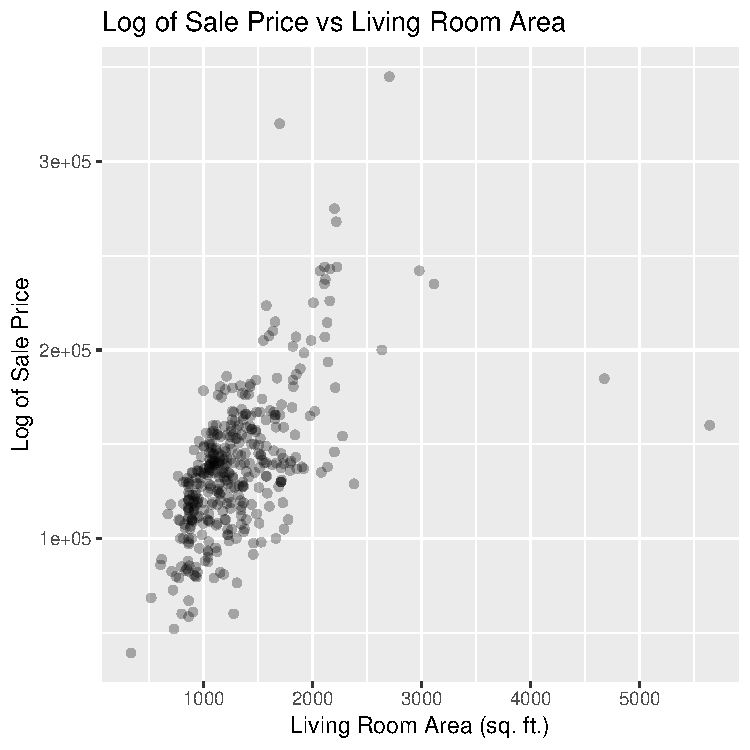
\includegraphics[width=0.45\linewidth]{HousePriceRegressionAnalysis_files/figure-latex/scatter-plot-1} 

}

\caption{Scatter Plot of Sale Price vs Living Room Area}\label{fig:scatter-plot}
\end{figure}

The images below show the scatter plots of log sale price vs living room
area (Figure \ref{fig:scatter-plots}). In the image on the right, the
scatter plot is shown for each neighborhood. In the image on the left
the observations for all three neighborhoods are included. In all cases,
a linear model appears to be reasonable to model this data.

\begin{figure}[htbp]

{\centering 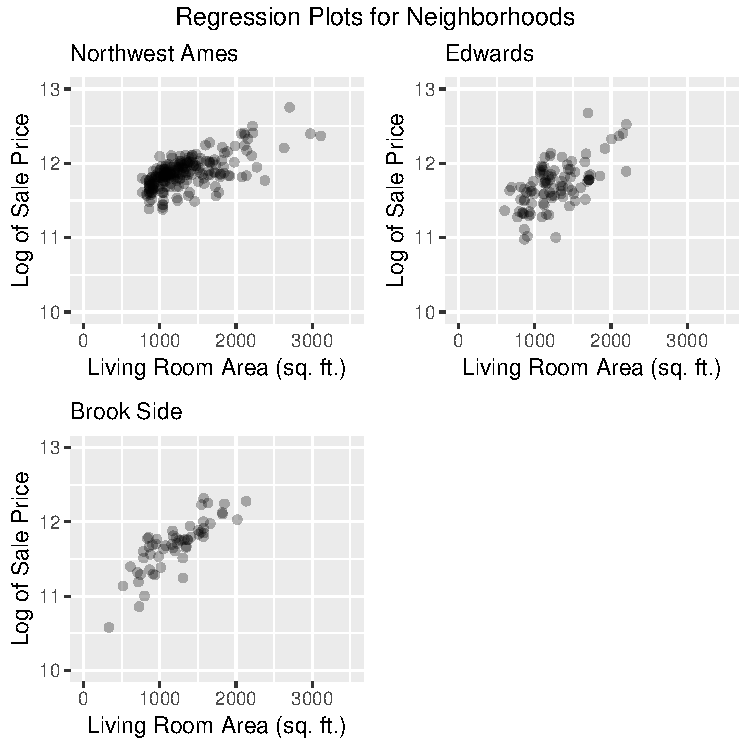
\includegraphics[width=0.45\linewidth]{HousePriceRegressionAnalysis_files/figure-latex/scatter-plots-1} 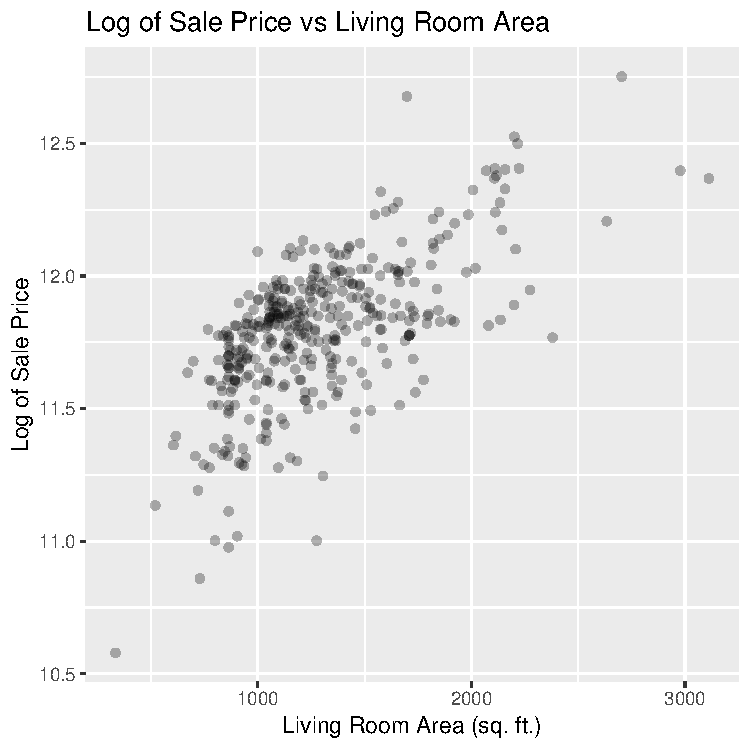
\includegraphics[width=0.45\linewidth]{HousePriceRegressionAnalysis_files/figure-latex/scatter-plots-2} 

}

\caption{Scatter Plots of Log of Sale Price vs Living Room Area}\label{fig:scatter-plots}
\end{figure}

\hypertarget{analysis-of-influential-points}{%
\subsection{Analysis of Influential
points}\label{analysis-of-influential-points}}

\label{appendix:infleu-points}

The two outlying observations with living room areas greater than 4000
sq. ft. appear to be from a different distribution than the main
dataset. Since these are partial sales, it is possible that the sale
prices do not reflect market value. For this reason, we will limit the
analysis to properities with less than 3500 sq. ft.
\ref{fig:infleu-points}

\begin{figure}[htbp]

{\centering 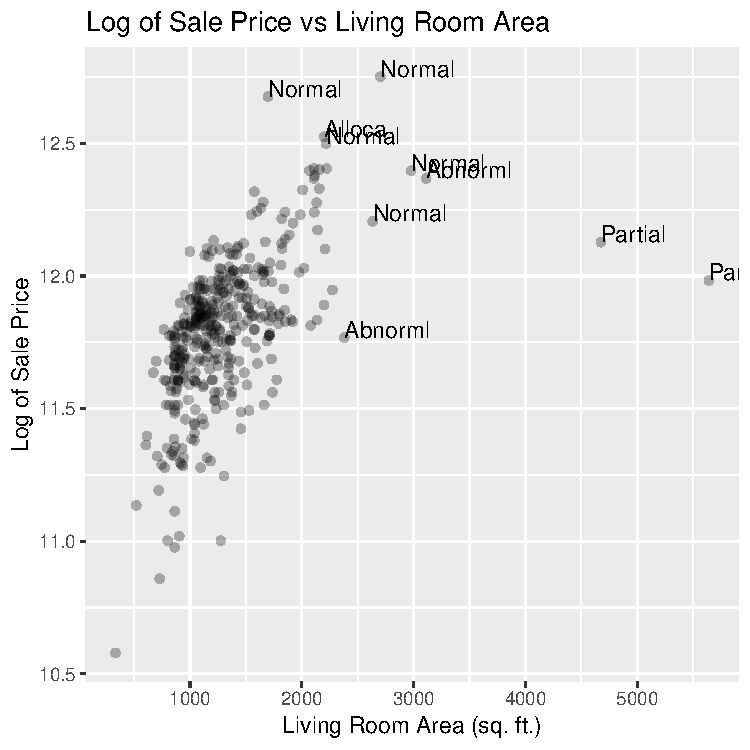
\includegraphics[width=0.5\linewidth]{HousePriceRegressionAnalysis_files/figure-latex/infleu-points-1} 

}

\caption{Influential Points}\label{fig:infleu-points}
\end{figure}

\newpage

\hypertarget{models-suggested-by-automated-selection}{%
\subsection{Models Suggested by Automated
Selection}\label{models-suggested-by-automated-selection}}

\hypertarget{forward-selection}{%
\subsubsection{Forward Selection}\label{forward-selection}}

\label{appendix:forSelection}

The model suggested by forward selection.

\begin{Shaded}
\begin{Highlighting}[]
\KeywordTok{log}\NormalTok{(SalePrice) }\OperatorTok{~}\StringTok{ }
\StringTok{              }\NormalTok{OverallQual }\OperatorTok{+}\StringTok{ }\NormalTok{GrLivArea }\OperatorTok{+}\StringTok{ }\NormalTok{Neighborhood }\OperatorTok{+}\StringTok{ }\NormalTok{BsmtFinSF1 }\OperatorTok{+}
\StringTok{              }\NormalTok{OverallCond }\OperatorTok{+}\StringTok{ }\NormalTok{YearBuilt }\OperatorTok{+}\StringTok{ }\NormalTok{TotalBsmtSF }\OperatorTok{+}\StringTok{ }\NormalTok{GarageCars }\OperatorTok{+}\StringTok{ }\NormalTok{MSZoning }\OperatorTok{+}
\StringTok{              }\NormalTok{SaleCondition }\OperatorTok{+}\StringTok{ }\NormalTok{BldgType }\OperatorTok{+}\StringTok{ }\NormalTok{Functional }\OperatorTok{+}\StringTok{ }\NormalTok{LotArea }\OperatorTok{+}\StringTok{ }\NormalTok{KitchenQual }\OperatorTok{+}
\StringTok{              }\NormalTok{BsmtExposure }\OperatorTok{+}\StringTok{ }\NormalTok{CentralAir }\OperatorTok{+}\StringTok{ }\NormalTok{Condition1 }\OperatorTok{+}\StringTok{ }\NormalTok{ScreenPorch }\OperatorTok{+}\StringTok{ }\NormalTok{BsmtFullBath }\OperatorTok{+}
\StringTok{              }\NormalTok{Heating }\OperatorTok{+}\StringTok{ }\NormalTok{Fireplaces }\OperatorTok{+}\StringTok{ }\NormalTok{YearRemodAdd }\OperatorTok{+}\StringTok{ }\NormalTok{Exterior1st }\OperatorTok{+}\StringTok{ }\NormalTok{GarageQual }\OperatorTok{+}
\StringTok{              }\NormalTok{WoodDeckSF }\OperatorTok{+}\StringTok{ }\NormalTok{SaleType }\OperatorTok{+}\StringTok{ }\NormalTok{OpenPorchSF }\OperatorTok{+}\StringTok{ }\NormalTok{HeatingQC }\OperatorTok{+}\StringTok{ }\NormalTok{LotConfig }\OperatorTok{+}
\StringTok{              }\NormalTok{EnclosedPorch }\OperatorTok{+}\StringTok{ }\NormalTok{ExterCond }\OperatorTok{+}\StringTok{ }\NormalTok{PoolQC }\OperatorTok{+}\StringTok{ }\NormalTok{Foundation }\OperatorTok{+}\StringTok{ }\NormalTok{LandSlope }\OperatorTok{+}
\StringTok{              }\NormalTok{RoofMatl }\OperatorTok{+}\StringTok{ }\NormalTok{GarageArea }\OperatorTok{+}\StringTok{ }\NormalTok{MasVnrType }\OperatorTok{+}\StringTok{ }\NormalTok{HalfBath }\OperatorTok{+}\StringTok{ }\NormalTok{PoolArea }\OperatorTok{+}
\StringTok{              `}\DataTypeTok{3SsnPorch}\StringTok{`} \OperatorTok{+}\StringTok{ }\NormalTok{Street }\OperatorTok{+}\StringTok{ }\NormalTok{KitchenAbvGr }\OperatorTok{+}\StringTok{ }\NormalTok{GarageCond }\OperatorTok{+}\StringTok{ }\NormalTok{FullBath }\OperatorTok{+}
\StringTok{              }\NormalTok{BsmtQual }\OperatorTok{+}\StringTok{ }\NormalTok{BsmtFinSF2}
\end{Highlighting}
\end{Shaded}

\hypertarget{backward-selection}{%
\subsubsection{Backward Selection}\label{backward-selection}}

\label{appendix:backSelection}

\begin{Shaded}
\begin{Highlighting}[]
\KeywordTok{log}\NormalTok{(SalePrice) }\OperatorTok{~}\StringTok{ }
\StringTok{           }\NormalTok{MSZoning }\OperatorTok{+}\StringTok{ }\NormalTok{LotArea }\OperatorTok{+}\StringTok{ }\NormalTok{Street }\OperatorTok{+}\StringTok{ }\NormalTok{LotConfig }\OperatorTok{+}\StringTok{ }\NormalTok{LandSlope }\OperatorTok{+}
\StringTok{           }\NormalTok{Neighborhood }\OperatorTok{+}\StringTok{ }\NormalTok{Condition1 }\OperatorTok{+}\StringTok{ }\NormalTok{Condition2 }\OperatorTok{+}\StringTok{ }\NormalTok{BldgType }\OperatorTok{+}\StringTok{ }\NormalTok{OverallQual }\OperatorTok{+}
\StringTok{           }\NormalTok{OverallCond }\OperatorTok{+}\StringTok{ }\NormalTok{YearBuilt }\OperatorTok{+}\StringTok{ }\NormalTok{YearRemodAdd }\OperatorTok{+}\StringTok{ }\NormalTok{RoofStyle }\OperatorTok{+}\StringTok{ }\NormalTok{RoofMatl }\OperatorTok{+}
\StringTok{           }\NormalTok{Exterior1st }\OperatorTok{+}\StringTok{ }\NormalTok{MasVnrType }\OperatorTok{+}\StringTok{ }\NormalTok{ExterCond }\OperatorTok{+}\StringTok{ }\NormalTok{Foundation }\OperatorTok{+}\StringTok{ }\NormalTok{BsmtQual }\OperatorTok{+}
\StringTok{           }\NormalTok{BsmtCond }\OperatorTok{+}\StringTok{ }\NormalTok{BsmtExposure }\OperatorTok{+}\StringTok{ }\NormalTok{BsmtFinSF1 }\OperatorTok{+}\StringTok{ }\NormalTok{BsmtFinSF2 }\OperatorTok{+}\StringTok{ }\NormalTok{BsmtUnfSF }\OperatorTok{+}
\StringTok{           }\NormalTok{Heating }\OperatorTok{+}\StringTok{ }\NormalTok{HeatingQC }\OperatorTok{+}\StringTok{ }\NormalTok{CentralAir }\OperatorTok{+}\StringTok{ `}\DataTypeTok{1stFlrSF}\StringTok{`} \OperatorTok{+}\StringTok{ `}\DataTypeTok{2ndFlrSF}\StringTok{`} \OperatorTok{+}
\StringTok{           }\NormalTok{LowQualFinSF }\OperatorTok{+}\StringTok{ }\NormalTok{BsmtFullBath }\OperatorTok{+}\StringTok{ }\NormalTok{FullBath }\OperatorTok{+}\StringTok{ }\NormalTok{HalfBath }\OperatorTok{+}\StringTok{ }\NormalTok{KitchenAbvGr }\OperatorTok{+}
\StringTok{           }\NormalTok{KitchenQual }\OperatorTok{+}\StringTok{ }\NormalTok{Functional }\OperatorTok{+}\StringTok{ }\NormalTok{Fireplaces }\OperatorTok{+}\StringTok{ }\NormalTok{GarageCars }\OperatorTok{+}\StringTok{ }\NormalTok{GarageArea }\OperatorTok{+}
\StringTok{           }\NormalTok{GarageQual }\OperatorTok{+}\StringTok{ }\NormalTok{GarageCond }\OperatorTok{+}\StringTok{ }\NormalTok{WoodDeckSF }\OperatorTok{+}\StringTok{ }\NormalTok{OpenPorchSF }\OperatorTok{+}\StringTok{ }\NormalTok{EnclosedPorch }\OperatorTok{+}
\StringTok{           `}\DataTypeTok{3SsnPorch}\StringTok{`} \OperatorTok{+}\StringTok{ }\NormalTok{ScreenPorch }\OperatorTok{+}\StringTok{ }\NormalTok{PoolArea }\OperatorTok{+}\StringTok{ }\NormalTok{PoolQC }\OperatorTok{+}\StringTok{ }\NormalTok{SaleType }\OperatorTok{+}
\StringTok{           }\NormalTok{SaleCondition}
\end{Highlighting}
\end{Shaded}

\newpage

\hypertarget{stepwise-selection}{%
\subsubsection{Stepwise Selection}\label{stepwise-selection}}

\label{appendix:stepWSelection}

\begin{Shaded}
\begin{Highlighting}[]
\KeywordTok{log}\NormalTok{(SalePrice) }\OperatorTok{~}\StringTok{ }
\StringTok{           }\NormalTok{MSZoning }\OperatorTok{+}\StringTok{ }\NormalTok{LotArea }\OperatorTok{+}\StringTok{ }\NormalTok{Street }\OperatorTok{+}\StringTok{ }\NormalTok{LotConfig }\OperatorTok{+}\StringTok{ }\NormalTok{LandSlope }\OperatorTok{+}
\StringTok{           }\NormalTok{Neighborhood }\OperatorTok{+}\StringTok{ }\NormalTok{Condition1 }\OperatorTok{+}\StringTok{ }\NormalTok{Condition2 }\OperatorTok{+}\StringTok{ }\NormalTok{BldgType }\OperatorTok{+}\StringTok{ }\NormalTok{OverallQual }\OperatorTok{+}
\StringTok{           }\NormalTok{OverallCond }\OperatorTok{+}\StringTok{ }\NormalTok{YearBuilt }\OperatorTok{+}\StringTok{ }\NormalTok{YearRemodAdd }\OperatorTok{+}\StringTok{ }\NormalTok{RoofStyle }\OperatorTok{+}\StringTok{ }\NormalTok{RoofMatl }\OperatorTok{+}
\StringTok{           }\NormalTok{Exterior1st }\OperatorTok{+}\StringTok{ }\NormalTok{MasVnrType }\OperatorTok{+}\StringTok{ }\NormalTok{ExterCond }\OperatorTok{+}\StringTok{ }\NormalTok{Foundation }\OperatorTok{+}\StringTok{ }\NormalTok{BsmtQual }\OperatorTok{+}
\StringTok{           }\NormalTok{BsmtCond }\OperatorTok{+}\StringTok{ }\NormalTok{BsmtExposure }\OperatorTok{+}\StringTok{ }\NormalTok{BsmtFinSF1 }\OperatorTok{+}\StringTok{ }\NormalTok{BsmtFinSF2 }\OperatorTok{+}\StringTok{ }\NormalTok{BsmtUnfSF }\OperatorTok{+}
\StringTok{           }\NormalTok{Heating }\OperatorTok{+}\StringTok{ }\NormalTok{HeatingQC }\OperatorTok{+}\StringTok{ }\NormalTok{CentralAir }\OperatorTok{+}\StringTok{ `}\DataTypeTok{1stFlrSF}\StringTok{`} \OperatorTok{+}\StringTok{ `}\DataTypeTok{2ndFlrSF}\StringTok{`} \OperatorTok{+}
\StringTok{           }\NormalTok{LowQualFinSF }\OperatorTok{+}\StringTok{ }\NormalTok{BsmtFullBath }\OperatorTok{+}\StringTok{ }\NormalTok{FullBath }\OperatorTok{+}\StringTok{ }\NormalTok{HalfBath }\OperatorTok{+}\StringTok{ }\NormalTok{KitchenAbvGr }\OperatorTok{+}
\StringTok{           }\NormalTok{KitchenQual }\OperatorTok{+}\StringTok{ }\NormalTok{Functional }\OperatorTok{+}\StringTok{ }\NormalTok{Fireplaces }\OperatorTok{+}\StringTok{ }\NormalTok{GarageCars }\OperatorTok{+}\StringTok{ }\NormalTok{GarageArea }\OperatorTok{+}
\StringTok{           }\NormalTok{GarageQual }\OperatorTok{+}\StringTok{ }\NormalTok{GarageCond }\OperatorTok{+}\StringTok{ }\NormalTok{WoodDeckSF }\OperatorTok{+}\StringTok{ }\NormalTok{OpenPorchSF }\OperatorTok{+}\StringTok{ }\NormalTok{EnclosedPorch }\OperatorTok{+}
\StringTok{           `}\DataTypeTok{3SsnPorch}\StringTok{`} \OperatorTok{+}\StringTok{ }\NormalTok{ScreenPorch }\OperatorTok{+}\StringTok{ }\NormalTok{PoolArea }\OperatorTok{+}\StringTok{ }\NormalTok{PoolQC }\OperatorTok{+}\StringTok{ }\NormalTok{SaleType }\OperatorTok{+}
\StringTok{           }\NormalTok{SaleCondition}
\end{Highlighting}
\end{Shaded}

\hypertarget{custom-model}{%
\subsubsection{Custom Model}\label{custom-model}}

\label{appendix:customSelection}

\begin{Shaded}
\begin{Highlighting}[]
\KeywordTok{log}\NormalTok{(SalePrice) }\OperatorTok{~}\StringTok{ }
\StringTok{            }\NormalTok{BsmtUnfSF }\OperatorTok{+}\StringTok{ }\NormalTok{CentralAir }\OperatorTok{+}\StringTok{ }\NormalTok{HalfBath }\OperatorTok{+}\StringTok{ }\NormalTok{KitchenQual }\OperatorTok{+}\StringTok{ }\NormalTok{Neighborhood }\OperatorTok{+}
\StringTok{            }\NormalTok{OverallCond }\OperatorTok{+}\StringTok{ }\NormalTok{OverallQual }\OperatorTok{+}\StringTok{ }\NormalTok{RoofMatl }\OperatorTok{+}\StringTok{ `}\DataTypeTok{1stFlrSF}\StringTok{`} \OperatorTok{+}\StringTok{ `}\DataTypeTok{2ndFlrSF}\StringTok{`} \OperatorTok{+}\StringTok{ }
\StringTok{            }\NormalTok{YearBuilt }\OperatorTok{+}\StringTok{ }\NormalTok{MSZoning}\OperatorTok{:}\NormalTok{Neighborhood }\OperatorTok{+}\StringTok{ }\NormalTok{YearBuilt}\OperatorTok{:}\NormalTok{Neighborhood}
\end{Highlighting}
\end{Shaded}

\hypertarget{kaggle-score}{%
\subsection{Kaggle Score}\label{kaggle-score}}

\label{appendix:kaggle}

The following image shows the result on Kaggle for the custom model.

\begin{center}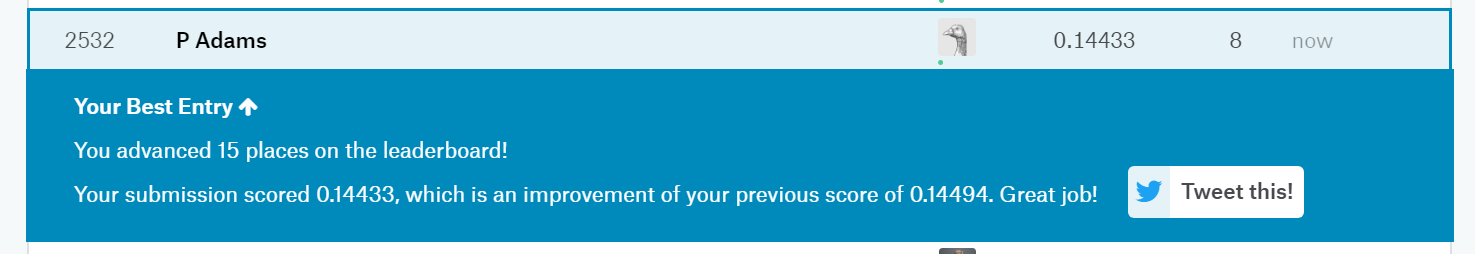
\includegraphics[width=0.9\linewidth]{./Evidence for Model Score on Kaggle} \end{center}

\newpage

\hypertarget{assumption-assessment-plots-for-automatic-selection-models}{%
\subsection{Assumption Assessment Plots for Automatic Selection
Models}\label{assumption-assessment-plots-for-automatic-selection-models}}

\label{appendix:assessmentPlots}

The following discussion applies to the assumption assessment for the
three models produced by automatic selection.

Based on the residuals vs.~fitted plot, there seems to be strong
linearity in the custom model, along with constant variance. The
standardized residuals do not appear to exhibit a discernible pattern,
indicating constant variance along the regression, or homoscedasticity.
However, there are three observations with unusually high residuals.

Based on the QQ plot, there is a small level of deviation on the ends of
the distribution of the errors, but for the most part, the errors adhere
to normality. The sample size should be sufficient to protect against
this non-normality.

Based on the standardized residuals vs.~leverage plot, only a few values
have high leverage and are outlying. Compared to the custom model
(Figure \ref{fig:custom-assumptions}), these diagnostic plots for these
models show a few more influential observations with high leverage.
However, these observations cannot be excluded from the model.

\begin{figure}[htbp]

{\centering \includegraphics[width=0.45\linewidth]{HousePriceRegressionAnalysis_files/figure-latex/forward-assumptions-1} \includegraphics[width=0.45\linewidth]{HousePriceRegressionAnalysis_files/figure-latex/forward-assumptions-2} 

}

\caption{Forward Selection Assumption Assessment Plots}\label{fig:forward-assumptions}
\end{figure}

\begin{figure}[htbp]

{\centering \includegraphics[width=0.45\linewidth]{HousePriceRegressionAnalysis_files/figure-latex/backward-selection-1} \includegraphics[width=0.45\linewidth]{HousePriceRegressionAnalysis_files/figure-latex/backward-selection-2} 

}

\caption{Backward Selection Assumption Assessment Plots}\label{fig:backward-selection}
\end{figure}

\begin{figure}[htbp]

{\centering \includegraphics[width=0.45\linewidth]{HousePriceRegressionAnalysis_files/figure-latex/stepwise-assimptions-1} \includegraphics[width=0.45\linewidth]{HousePriceRegressionAnalysis_files/figure-latex/stepwise-assimptions-2} 

}

\caption{Stepwise Selection Assumption Assessment Plots}\label{fig:stepwise-assimptions}
\end{figure}

\newpage

\hypertarget{r-code-for-analysis-1}{%
\subsection{R Code For Analysis 1}\label{r-code-for-analysis-1}}

\begin{Shaded}
\begin{Highlighting}[]
\CommentTok{### Compuational Setup}
\CommentTok{# libraries}
\KeywordTok{library}\NormalTok{(knitr)}
\KeywordTok{library}\NormalTok{(kableExtra)}
\KeywordTok{library}\NormalTok{(tidyverse)}
\KeywordTok{library}\NormalTok{(olsrr)}
\KeywordTok{library}\NormalTok{(gridExtra)}
\KeywordTok{library}\NormalTok{(caret)}
\KeywordTok{library}\NormalTok{(multcomp)}

\CommentTok{# load data}
\NormalTok{train <-}\StringTok{ }\KeywordTok{read_csv}\NormalTok{(}\StringTok{'./data/train.csv'}\NormalTok{)}
\NormalTok{test <-}\StringTok{ }\KeywordTok{read_csv}\NormalTok{(}\StringTok{'./data/test.csv'}\NormalTok{)}

\CommentTok{# set a random seed for repodicibility}
\KeywordTok{set.seed}\NormalTok{(}\DecValTok{123}\NormalTok{)}

\CommentTok{### Helper Code}

\CommentTok{#' Print Typical Regression Fit Plots}
\CommentTok{#' }
\CommentTok{#' @description}
\CommentTok{#' Plots QQ plot of residuals, histogram of residuals,}
\CommentTok{#' residuals vs predicted values, and studentized }
\CommentTok{#' residuals vs predicted values. Depends on tidyverse}
\CommentTok{#' and gridExtra packages being loaded.}
\CommentTok{#'}
\CommentTok{#' @param data The true values corresponding to the input.}
\CommentTok{#' @param model The predicted/fitted values of the model.}
\NormalTok{basic.fit.plots <-}\StringTok{ }\ControlFlowTok{function}\NormalTok{(data, model) \{}
    
    \CommentTok{# depends on}
    \KeywordTok{require}\NormalTok{(tidyverse)}
    \KeywordTok{require}\NormalTok{(gridExtra)}

    \CommentTok{# get predicted values}
\NormalTok{    data}\OperatorTok{$}\NormalTok{Predicted <-}\StringTok{ }\KeywordTok{predict}\NormalTok{(model, data)}
    \CommentTok{# get residuals}
\NormalTok{    data}\OperatorTok{$}\NormalTok{Resid <-}\StringTok{ }\NormalTok{model}\OperatorTok{$}\NormalTok{residuals}
    \CommentTok{# get studentized residuals}
\NormalTok{    data}\OperatorTok{$}\NormalTok{RStudent <-}\StringTok{ }\KeywordTok{rstudent}\NormalTok{(}\DataTypeTok{model =}\NormalTok{ model)}

    \CommentTok{# create qqplot of residuals with reference line}
\NormalTok{    qqplot.resid <-}\StringTok{ }\NormalTok{data }\OperatorTok\StringTok{ }
\StringTok{      }\KeywordTok{ggplot}\NormalTok{(}\KeywordTok{aes}\NormalTok{(}\DataTypeTok{sample =}\NormalTok{ Resid)) }\OperatorTok{+}
\StringTok{      }\KeywordTok{geom_qq}\NormalTok{() }\OperatorTok{+}\StringTok{ }\KeywordTok{geom_qq_line}\NormalTok{() }\OperatorTok{+}
\StringTok{      }\KeywordTok{labs}\NormalTok{(}\DataTypeTok{subtitle =} \StringTok{'QQ Plot of Residuals'}\NormalTok{,}
           \DataTypeTok{x =} \StringTok{'Theoretical Quantile'}\NormalTok{,}
           \DataTypeTok{y =} \StringTok{'Acutal Quantile'}\NormalTok{)}
    
    \CommentTok{# create histogram of residuals}
\NormalTok{    hist.resid <-}\StringTok{ }\NormalTok{data }\OperatorTok\StringTok{ }
\StringTok{      }\KeywordTok{ggplot}\NormalTok{(}\KeywordTok{aes}\NormalTok{(}\DataTypeTok{x =}\NormalTok{ Resid)) }\OperatorTok{+}
\StringTok{      }\KeywordTok{geom_histogram}\NormalTok{(}\DataTypeTok{bins =} \DecValTok{15}\NormalTok{) }\OperatorTok{+}\StringTok{ }
\StringTok{      }\KeywordTok{labs}\NormalTok{(}\DataTypeTok{subtitle =} \StringTok{'Histogram of Residuals'}\NormalTok{,}
           \DataTypeTok{x =} \StringTok{'Residuals'}\NormalTok{,}
           \DataTypeTok{y =} \StringTok{'Count'}\NormalTok{)}

    \CommentTok{# create scatter plot of residuals vs predicted values}
\NormalTok{    resid.vs.pred <-}\StringTok{ }\NormalTok{data }\OperatorTok\StringTok{ }
\StringTok{      }\KeywordTok{ggplot}\NormalTok{(}\KeywordTok{aes}\NormalTok{(}\DataTypeTok{x =}\NormalTok{ Predicted, }\DataTypeTok{y =}\NormalTok{ Resid)) }\OperatorTok{+}
\StringTok{      }\KeywordTok{geom_point}\NormalTok{() }\OperatorTok{+}
\StringTok{      }\KeywordTok{geom_abline}\NormalTok{(}\DataTypeTok{slope =} \DecValTok{0}\NormalTok{) }\OperatorTok{+}\StringTok{ }
\StringTok{      }\KeywordTok{labs}\NormalTok{(}\DataTypeTok{subtitle =} \StringTok{'Residuals vs Prediction'}\NormalTok{,}
           \DataTypeTok{x =} \StringTok{'Predicted Value'}\NormalTok{,}
           \DataTypeTok{y =} \StringTok{'Residual'}\NormalTok{)}

    \CommentTok{# create scatter plot of studentized }
    \CommentTok{# residuals vs predicted values}
\NormalTok{    rStud.vs.pred <-}\StringTok{ }\NormalTok{data }\OperatorTok\StringTok{ }
\StringTok{      }\KeywordTok{ggplot}\NormalTok{(}\KeywordTok{aes}\NormalTok{(}\DataTypeTok{x =}\NormalTok{ Predicted, }\DataTypeTok{y =}\NormalTok{ RStudent)) }\OperatorTok{+}
\StringTok{      }\KeywordTok{geom_point}\NormalTok{() }\OperatorTok{+}
\StringTok{      }\KeywordTok{geom_abline}\NormalTok{(}\DataTypeTok{slope =} \DecValTok{0}\NormalTok{) }\OperatorTok{+}\StringTok{ }
\StringTok{      }\KeywordTok{geom_abline}\NormalTok{(}\DataTypeTok{slope =} \DecValTok{0}\NormalTok{, }\DataTypeTok{intercept =} \DecValTok{-2}\NormalTok{) }\OperatorTok{+}\StringTok{ }
\StringTok{      }\KeywordTok{geom_abline}\NormalTok{(}\DataTypeTok{slope =} \DecValTok{0}\NormalTok{, }\DataTypeTok{intercept =} \DecValTok{2}\NormalTok{) }\OperatorTok{+}\StringTok{ }
\StringTok{      }\KeywordTok{labs}\NormalTok{(}\DataTypeTok{subtitle =} \StringTok{'RStudent vs Prediction'}\NormalTok{,}
           \DataTypeTok{x =} \StringTok{'Predicted Value'}\NormalTok{,}
           \DataTypeTok{y =} \StringTok{'RStudent'}\NormalTok{)}
    
    \CommentTok{# add all four plots to grid as}
    \CommentTok{# qqplot           histogram}
    \CommentTok{# resid vs pred    RStud vs pred}
    \KeywordTok{grid.arrange}\NormalTok{(qqplot.resid,}
\NormalTok{             hist.resid,}
\NormalTok{             resid.vs.pred,}
\NormalTok{             rStud.vs.pred, }
             \DataTypeTok{nrow =} \DecValTok{2}\NormalTok{,}
             \DataTypeTok{top =} \StringTok{'Fit Assessment Plots'}\NormalTok{)}
\NormalTok{\}}

\CommentTok{#' Creates dummy variables (columns) for given column}
\CommentTok{#'}
\CommentTok{#' @param data A dataframe.}
\CommentTok{#' @param column A categorical column in data.}
\CommentTok{#' @param reference A value in the column to use a reference.}
\CommentTok{#' @param as.onehot Set to TRUE to use onehot encoding.}
\CommentTok{#'}
\NormalTok{get.dummies <-}\StringTok{ }\ControlFlowTok{function}\NormalTok{(data, column, reference, }\DataTypeTok{as.onehot =} \OtherTok{FALSE}\NormalTok{) \{}
  \CommentTok{# get the levels of the factor in column}
\NormalTok{  lev <-}\StringTok{ }\KeywordTok{levels}\NormalTok{(data[[column]])}
  \CommentTok{# do not remove reference for onehot encoding}
  \ControlFlowTok{if}\NormalTok{ (}\OperatorTok{!}\NormalTok{as.onehot) \{}
    \CommentTok{# remove the reference value}
\NormalTok{    lev <-}\StringTok{ }\NormalTok{lev[lev }\OperatorTok{!=}\StringTok{ }\NormalTok{reference]}
\NormalTok{  \}}
  \CommentTok{# add encodings}
  \ControlFlowTok{for}\NormalTok{ (fct }\ControlFlowTok{in}\NormalTok{ lev)\{}
\NormalTok{    new_col <-}\StringTok{ }\KeywordTok{paste}\NormalTok{(column, fct, }\DataTypeTok{sep =} \StringTok{'_'}\NormalTok{)}
\NormalTok{    data[new_col] <-}\StringTok{ }\KeywordTok{as.numeric}\NormalTok{(data[, column] }\OperatorTok{==}\StringTok{ }\NormalTok{fct)}
    \KeywordTok{print}\NormalTok{(new_col)}
\NormalTok{  \}}
\NormalTok{  data}
\NormalTok{\}}

\CommentTok{#' Calculates PRESS from `caret` CV model}
\CommentTok{#'}
\CommentTok{#' @param model.cv Calculates press from a model }
\CommentTok{#' produced by `caret`}
\CommentTok{#'}
\NormalTok{PRESS.cv <-}\StringTok{ }\ControlFlowTok{function}\NormalTok{(model.cv) \{}
\NormalTok{  meanN <-}\StringTok{ }\DecValTok{0}
\NormalTok{  folds <-}\StringTok{ }\NormalTok{model.cv}\OperatorTok{$}\NormalTok{control}\OperatorTok{$}\NormalTok{index}
  \ControlFlowTok{for}\NormalTok{ (i }\ControlFlowTok{in} \KeywordTok{seq}\NormalTok{(}\DecValTok{1}\OperatorTok{:}\KeywordTok{length}\NormalTok{(folds)))\{}
\NormalTok{    meanN <-}\StringTok{ }\NormalTok{meanN }\OperatorTok{+}\StringTok{ }\KeywordTok{length}\NormalTok{(folds[[i]])}
\NormalTok{  \}}
\NormalTok{  meanN <-}\StringTok{ }\NormalTok{meanN }\OperatorTok{/}\StringTok{ }\KeywordTok{length}\NormalTok{(folds)}
\NormalTok{  meanN }\OperatorTok{*}\StringTok{ }\NormalTok{((model.cv}\OperatorTok{$}\NormalTok{results}\OperatorTok{$}\NormalTok{RMSE)}\OperatorTok{^}\DecValTok{2}\NormalTok{)}
\NormalTok{\}}

\CommentTok{### plots of log of sale price ~ living room area}

\CommentTok{# create scatter plot for northwest ames}
\NormalTok{regplot.names <-}\StringTok{ }\NormalTok{train }\OperatorTok\StringTok{ }\KeywordTok{filter}\NormalTok{(Neighborhood }\OperatorTok{==}\StringTok{ 'NAmes'}\NormalTok{) }\OperatorTok
\StringTok{  }\KeywordTok{ggplot}\NormalTok{(}\KeywordTok{aes}\NormalTok{(}\DataTypeTok{x =}\NormalTok{ (GrLivArea), }\DataTypeTok{y =} \KeywordTok{log}\NormalTok{(SalePrice))) }\OperatorTok{+}
\StringTok{  }\KeywordTok{geom_point}\NormalTok{(}\DataTypeTok{alpha =} \FloatTok{0.3}\NormalTok{) }\OperatorTok{+}
\StringTok{  }\KeywordTok{ylim}\NormalTok{(}\DecValTok{10}\NormalTok{, }\DecValTok{13}\NormalTok{) }\OperatorTok{+}
\StringTok{  }\KeywordTok{xlim}\NormalTok{(}\DecValTok{0}\NormalTok{, }\DecValTok{3500}\NormalTok{) }\OperatorTok{+}
\StringTok{  }\KeywordTok{labs}\NormalTok{(}\DataTypeTok{subtitle =} \StringTok{'Northwest Ames'}\NormalTok{, }
       \DataTypeTok{y =} \StringTok{'Log of Sale Price'}\NormalTok{, }\DataTypeTok{x =} \StringTok{'Living Room Area (sq. ft.)'}\NormalTok{)}

\CommentTok{# create scatter plot for edwards}
\NormalTok{regplot.ed <-}\StringTok{ }\NormalTok{train }\OperatorTok
\StringTok{  }\KeywordTok{filter}\NormalTok{(GrLivArea }\OperatorTok{<}\StringTok{ }\DecValTok{4000}\NormalTok{) }\OperatorTok
\StringTok{  }\KeywordTok{filter}\NormalTok{(Neighborhood }\OperatorTok{==}\StringTok{ 'Edwards'}\NormalTok{) }\OperatorTok
\StringTok{  }\KeywordTok{ggplot}\NormalTok{(}\KeywordTok{aes}\NormalTok{(}\DataTypeTok{x =}\NormalTok{ (GrLivArea), }\DataTypeTok{y =} \KeywordTok{log}\NormalTok{(SalePrice))) }\OperatorTok{+}
\StringTok{  }\KeywordTok{geom_point}\NormalTok{(}\DataTypeTok{alpha =} \FloatTok{0.3}\NormalTok{) }\OperatorTok{+}
\StringTok{  }\KeywordTok{ylim}\NormalTok{(}\DecValTok{10}\NormalTok{, }\DecValTok{13}\NormalTok{) }\OperatorTok{+}
\StringTok{  }\KeywordTok{xlim}\NormalTok{(}\DecValTok{0}\NormalTok{, }\DecValTok{3500}\NormalTok{) }\OperatorTok{+}
\StringTok{  }\KeywordTok{labs}\NormalTok{(}\DataTypeTok{subtitle =} \StringTok{'Edwards'}\NormalTok{, }
       \DataTypeTok{y =} \StringTok{'Log of Sale Price'}\NormalTok{, }\DataTypeTok{x =} \StringTok{'Living Room Area (sq. ft.)'}\NormalTok{)}

\CommentTok{# create regression plot for brookside}
\NormalTok{regplot.brk <-}\StringTok{ }\NormalTok{train }\OperatorTok\StringTok{ }\KeywordTok{filter}\NormalTok{(Neighborhood }\OperatorTok{==}\StringTok{ 'BrkSide'}\NormalTok{) }\OperatorTok
\StringTok{  }\KeywordTok{ggplot}\NormalTok{(}\KeywordTok{aes}\NormalTok{(}\DataTypeTok{x =}\NormalTok{ (GrLivArea), }\DataTypeTok{y =} \KeywordTok{log}\NormalTok{(SalePrice))) }\OperatorTok{+}
\StringTok{  }\KeywordTok{geom_point}\NormalTok{(}\DataTypeTok{alpha =} \FloatTok{0.3}\NormalTok{) }\OperatorTok{+}
\StringTok{  }\KeywordTok{ylim}\NormalTok{(}\DecValTok{10}\NormalTok{, }\DecValTok{13}\NormalTok{) }\OperatorTok{+}
\StringTok{  }\KeywordTok{xlim}\NormalTok{(}\DecValTok{0}\NormalTok{, }\DecValTok{3500}\NormalTok{) }\OperatorTok{+}
\StringTok{  }\KeywordTok{labs}\NormalTok{(}\DataTypeTok{subtitle =} \StringTok{'Brook Side'}\NormalTok{, }
       \DataTypeTok{y =} \StringTok{'Log of Sale Price'}\NormalTok{, }\DataTypeTok{x =} \StringTok{'Living Room Area (sq. ft.)'}\NormalTok{)}

\CommentTok{# add the scatter plots for the neighborhood into a single plot}
\KeywordTok{grid.arrange}\NormalTok{(regplot.names,regplot.ed,regplot.brk, }\DataTypeTok{nrow =} \DecValTok{2}\NormalTok{,}
             \DataTypeTok{top =} \StringTok{'Regression Plots for Neighborhoods'}\NormalTok{)}

\CommentTok{# scatter plot of observations from all three neighborhoods}
\NormalTok{train }\OperatorTok\StringTok{ }
\StringTok{  }\KeywordTok{filter}\NormalTok{(GrLivArea }\OperatorTok{<}\StringTok{ }\DecValTok{4000}\NormalTok{) }\OperatorTok
\StringTok{  }\KeywordTok{ggplot}\NormalTok{(}\KeywordTok{aes}\NormalTok{(}\DataTypeTok{x =}\NormalTok{ (GrLivArea), }\DataTypeTok{y =} \KeywordTok{log}\NormalTok{(SalePrice))) }\OperatorTok{+}
\StringTok{  }\KeywordTok{geom_point}\NormalTok{(}\DataTypeTok{alpha =} \FloatTok{0.3}\NormalTok{) }\OperatorTok{+}
\StringTok{  }\KeywordTok{labs}\NormalTok{(}\DataTypeTok{title =} \StringTok{'Log of Sale Price vs Living Room Area'}\NormalTok{, }
       \DataTypeTok{y =} \StringTok{'Log of Sale Price'}\NormalTok{, }\DataTypeTok{x =} \StringTok{'Living Room Area (sq. ft.)'}\NormalTok{)}

\CommentTok{### Filter data for analysis 1}

\NormalTok{train <-}\StringTok{ }\NormalTok{train }\OperatorTok\StringTok{ }
\StringTok{  }\KeywordTok{filter}\NormalTok{(Neighborhood }\OperatorTok\StringTok{ }\KeywordTok{c}\NormalTok{(}\StringTok{"Edwards"}\NormalTok{, }\StringTok{"BrkSide"}\NormalTok{, }\StringTok{"NAmes"}\NormalTok{))}
\NormalTok{train}\OperatorTok{$}\NormalTok{Neighborhood <-}\StringTok{ }\KeywordTok{as.factor}\NormalTok{(train}\OperatorTok{$}\NormalTok{Neighborhood)}

\CommentTok{# create dummy variables with Neighborhood == 'Edwards' as reference}
\NormalTok{train <-}\StringTok{ }\KeywordTok{get.dummies}\NormalTok{(train, }\StringTok{"Neighborhood"}\NormalTok{, }\DataTypeTok{reference =} \StringTok{'Edwards'}\NormalTok{)}

\CommentTok{# remove suspect points from training data}
\NormalTok{train.mod <-}\StringTok{ }\NormalTok{train }\OperatorTok\StringTok{ }\KeywordTok{filter}\NormalTok{(GrLivArea }\OperatorTok{<}\StringTok{ }\DecValTok{4000}\NormalTok{)}

\CommentTok{#### Extra Sum of Squares}

\CommentTok{# full model formula}
\NormalTok{model.formula =}\StringTok{ }\KeywordTok{log}\NormalTok{(SalePrice) }\OperatorTok{~}\StringTok{ }\NormalTok{(GrLivArea) }\OperatorTok{+}\StringTok{ }
\StringTok{     }\NormalTok{Neighborhood_BrkSide }\OperatorTok{+}\StringTok{ }
\StringTok{     }\NormalTok{Neighborhood_NAmes }\OperatorTok{+}
\StringTok{     }\NormalTok{(GrLivArea) }\OperatorTok{*}\StringTok{ }\NormalTok{Neighborhood_BrkSide }\OperatorTok{+}\StringTok{ }
\StringTok{     }\NormalTok{(GrLivArea) }\OperatorTok{*}\StringTok{ }\NormalTok{Neighborhood_NAmes}
\CommentTok{# reduced model formula}
\NormalTok{model.reduced.formula =}\StringTok{ }\KeywordTok{log}\NormalTok{(SalePrice) }\OperatorTok{~}\StringTok{ }\NormalTok{(GrLivArea) }\OperatorTok{+}\StringTok{ }
\StringTok{     }\NormalTok{Neighborhood_BrkSide }\OperatorTok{+}\StringTok{ }
\StringTok{     }\NormalTok{Neighborhood_NAmes}

\CommentTok{# fit models}
\NormalTok{model <-}\StringTok{ }\KeywordTok{lm}\NormalTok{(}\DataTypeTok{formula =}\NormalTok{ model.formula, }\DataTypeTok{data =}\NormalTok{ train.mod)}
\NormalTok{model.reduced <-}\StringTok{ }\KeywordTok{lm}\NormalTok{(}\DataTypeTok{formula =}\NormalTok{ model.reduced.formula, }\DataTypeTok{data =}\NormalTok{ train.mod)}
\CommentTok{# ESS test on models}
\KeywordTok{anova}\NormalTok{(model.reduced, model)}

\CommentTok{### Assessment plots}

\CommentTok{# create plots of residuals}
\KeywordTok{basic.fit.plots}\NormalTok{(train.mod, model)}
\CommentTok{# create leverage / outlier plot}
\KeywordTok{ols_plot_resid_lev}\NormalTok{(model)}

\CommentTok{### cross validation}

\CommentTok{## cross validate the full model}

\CommentTok{# Set up repeated k-fold cross-validation}
\NormalTok{train.control <-}\StringTok{ }\KeywordTok{trainControl}\NormalTok{(}\DataTypeTok{method =} \StringTok{"cv"}\NormalTok{, }\DataTypeTok{number =} \DecValTok{10}\NormalTok{)}
\CommentTok{# Train the model}
\NormalTok{model.cv <-}\StringTok{ }\KeywordTok{train}\NormalTok{(model.formula, }
                    \DataTypeTok{data =}\NormalTok{ train.mod,}
                    \DataTypeTok{method =} \StringTok{'lm'}\NormalTok{,}
                    \DataTypeTok{trControl =}\NormalTok{ train.control)}
\CommentTok{# print model summary}
\NormalTok{model.cv}

\CommentTok{# get the CV results}
\NormalTok{res <-}\StringTok{ }\NormalTok{model.cv}\OperatorTok{$}\NormalTok{results}

\CommentTok{# get cross-validated PRESS statistic}
\NormalTok{PCV <-}\StringTok{ }\KeywordTok{PRESS.cv}\NormalTok{(model.cv)}

\CommentTok{## cross validate the reduced model}

\CommentTok{# Set up repeated k-fold cross-validation}
\NormalTok{train.control <-}\StringTok{ }\KeywordTok{trainControl}\NormalTok{(}\DataTypeTok{method =} \StringTok{"cv"}\NormalTok{, }\DataTypeTok{number =} \DecValTok{10}\NormalTok{)}
\CommentTok{# Train the model}
\NormalTok{model.reduced.cv <-}\StringTok{ }\KeywordTok{train}\NormalTok{(model.reduced.formula, }
                    \DataTypeTok{data =}\NormalTok{ train.mod,}
                    \DataTypeTok{method =} \StringTok{'lm'}\NormalTok{,}
                    \DataTypeTok{trControl =}\NormalTok{ train.control)}
\CommentTok{# print model summary}
\NormalTok{model.reduced.cv}

\CommentTok{# get the CV results}
\NormalTok{res.red <-}\StringTok{ }\NormalTok{model.reduced.cv}\OperatorTok{$}\NormalTok{results}

\CommentTok{# get cross-validated PRESS statistic}
\NormalTok{PCV.red <-}\StringTok{ }\KeywordTok{PRESS.cv}\NormalTok{(model.reduced.cv)}

\CommentTok{# print accuracy metrics to md table}
\KeywordTok{kable}\NormalTok{(}\KeywordTok{data.frame}\NormalTok{(}\StringTok{'Model'}\NormalTok{ =}\StringTok{ }\KeywordTok{c}\NormalTok{(}\StringTok{'Full Model'}\NormalTok{, }\StringTok{'Reduced Model'}\NormalTok{), }
                 \StringTok{'RMSE'}\NormalTok{=}\KeywordTok{c}\NormalTok{(res}\OperatorTok{$}\NormalTok{RMSE, res.red}\OperatorTok{$}\NormalTok{RMSE),}
                 \StringTok{'CV Press'}\NormalTok{=}\KeywordTok{c}\NormalTok{(PCV, PCV.red),}
                 \StringTok{'Adjused R Squared'}\NormalTok{=}\KeywordTok{c}\NormalTok{(res}\OperatorTok{$}\NormalTok{Rsquared, res.red}\OperatorTok{$}\NormalTok{Rsquared)),}
      \StringTok{"latex"}\NormalTok{, }\DataTypeTok{booktabs =}\NormalTok{ T)  }\OperatorTok
\StringTok{  }\KeywordTok{kable_styling}\NormalTok{(}\DataTypeTok{position =} \StringTok{"center"}\NormalTok{)}

\CommentTok{### get the parameters from the CV'ed model}

\CommentTok{# extract the model estimates from the model summary}
\NormalTok{sm <-}\StringTok{ }\KeywordTok{summary}\NormalTok{(model)}
\NormalTok{sm.coe <-}\StringTok{ }\NormalTok{sm}\OperatorTok{$}\NormalTok{coefficients}
\CommentTok{# get the CIs for the coefficients}
\NormalTok{model.conf <-}\StringTok{ }\KeywordTok{confint}\NormalTok{(model)}

\CommentTok{# print model estimates to md / latex table}
\CommentTok{# extract the params and put into a dataframe}
\KeywordTok{kable}\NormalTok{(}\KeywordTok{data.frame}\NormalTok{(}\StringTok{'Parameter'}\NormalTok{ =}\StringTok{ }\KeywordTok{c}\NormalTok{(}\StringTok{'Intercept'}\NormalTok{, }\StringTok{'GrLivArea'}\NormalTok{, }
                                 \StringTok{'Neighborhood_BrkSide'}\NormalTok{, }\StringTok{'Neighborhood_NAmes'}\NormalTok{, }
                                 \StringTok{'GrLivArea:Neighborhood_BrkSide'}\NormalTok{, }
                                 \StringTok{'GrLivArea:Neighborhood_NAmes '}\NormalTok{), }
                 \StringTok{'Estimate'}\NormalTok{=}\KeywordTok{c}\NormalTok{(sm.coe[[}\DecValTok{1}\NormalTok{]],sm.coe[[}\DecValTok{2}\NormalTok{]],sm.coe[[}\DecValTok{3}\NormalTok{]],}
\NormalTok{                              sm.coe[[}\DecValTok{4}\NormalTok{]],sm.coe[[}\DecValTok{5}\NormalTok{]],sm.coe[[}\DecValTok{6}\NormalTok{]]),}
                 \StringTok{'CI Lower'}\NormalTok{ =}\StringTok{ }\KeywordTok{c}\NormalTok{(model.conf[[}\DecValTok{1}\NormalTok{]],model.conf[[}\DecValTok{2}\NormalTok{]],model.conf[[}\DecValTok{3}\NormalTok{]],}
\NormalTok{                                model.conf[[}\DecValTok{4}\NormalTok{]],model.conf[[}\DecValTok{5}\NormalTok{]],model.conf[[}\DecValTok{6}\NormalTok{]]),}
                 \StringTok{'CI Upper'}\NormalTok{ =}\StringTok{ }\KeywordTok{c}\NormalTok{(model.conf[[}\DecValTok{1}\NormalTok{,}\DecValTok{2}\NormalTok{]],model.conf[[}\DecValTok{1}\NormalTok{,}\DecValTok{2}\NormalTok{]],model.conf[[}\DecValTok{3}\NormalTok{,}\DecValTok{2}\NormalTok{]],}
\NormalTok{                                model.conf[[}\DecValTok{4}\NormalTok{,}\DecValTok{2}\NormalTok{]],model.conf[[}\DecValTok{5}\NormalTok{,}\DecValTok{2}\NormalTok{]],model.conf[[}\DecValTok{6}\NormalTok{,}\DecValTok{2}\NormalTok{]])),}
      \StringTok{"latex"}\NormalTok{, }\DataTypeTok{booktabs =}\NormalTok{ T)  }\OperatorTok
\StringTok{  }\KeywordTok{kable_styling}\NormalTok{(}\DataTypeTok{position =} \StringTok{"center"}\NormalTok{)}

\CommentTok{# summary of model to get overall test}
\KeywordTok{summary}\NormalTok{(}\KeywordTok{lm}\NormalTok{(model.formula, }\DataTypeTok{data =}\NormalTok{ train.mod))}

\CommentTok{## Calculate CIs of slopes not in standard table}

\CommentTok{# get CI for Northwest Ames}
\KeywordTok{confint}\NormalTok{(}\KeywordTok{glht}\NormalTok{(model, }\DataTypeTok{linfct =} \StringTok{"GrLivArea + GrLivArea:Neighborhood_NAmes = 1"}\NormalTok{))}

\CommentTok{# get CI for Brookside}
\KeywordTok{confint}\NormalTok{(}\KeywordTok{glht}\NormalTok{(model, }\DataTypeTok{linfct =} \StringTok{"GrLivArea + GrLivArea:Neighborhood_BrkSide = 1"}\NormalTok{))}
\end{Highlighting}
\end{Shaded}

\newpage

\hypertarget{r-code-for-analysis-2}{%
\subsection{R Code For Analysis 2}\label{r-code-for-analysis-2}}

\begin{Shaded}
\begin{Highlighting}[]

\end{Highlighting}
\end{Shaded}

\newpage

\renewcommand\refname{References}
\bibliography{references.bib}


\end{document}
